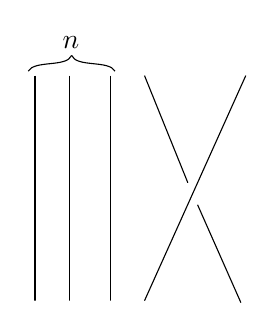
\begin{tikzpicture}[yscale=-1,scale=0.02,baseline={([yshift=-.5ex]current bounding box.center)}]
\begin{scope}[shift={(0.00mm,719.29mm)}]
% path id='path3355'
% path spec='m 199.97069,-371.51247 0,1427.27197 0,-2.302'
\draw [fill=none,draw=black] (199.97mm,-371.51mm)
-- ++(0.00mm,1427.27mm)
-- ++(0.00mm,-2.30mm)
;
% path id='path3357'
% path spec='m 419.98033,-371.51247 0,1427.27197 0,-2.302'
\draw [fill=none,draw=black] (419.98mm,-371.51mm)
-- ++(0.00mm,1427.27mm)
-- ++(0.00mm,-2.30mm)
;
% path id='path3359'
% path spec='m 679.99172,-371.51247 0,1427.27197 0,-2.302'
\draw [fill=none,draw=black] (679.99mm,-371.51mm)
-- ++(0.00mm,1427.27mm)
-- ++(0.00mm,-2.30mm)
;
% path id='path3361'
% path spec='M 895.21456,1056.8365 1538.0061,-371.97018'
\draw [fill=none,draw=black] (895.21mm,1056.84mm)
-- (1538.01mm,-371.97mm)
;
% path id='path3363'
% path spec='M 895.21456,-371.97015 1170.2945,308.0503'
\draw [fill=none,draw=black] (895.21mm,-371.97mm)
-- (1170.29mm,308.05mm)
;
% path id='path3365'
% path spec='m 1231.9603,447.66194 275.08,621.41976'
\draw [fill=none,draw=black] (1231.96mm,447.66mm)
-- ++(275.08mm,621.42mm)
;
% path id='path3367'
% path spec='m 156.96417,-400.42251 c 41.29201,-71.81739 243.8386,-22.30256 275.78464,-99.80392'
\draw [fill=none,draw=black] (156.96mm,-400.42mm)
.. controls ++(41.29mm,-71.82mm) and ++(-31.95mm,77.50mm) .. ++(275.78mm,-99.80mm)
;
% path id='path3369'
% path spec='m 708.3568,-400.307 c -41.292,-71.81738 -243.8386,-22.30256 -275.78464,-99.80392'
\draw [fill=none,draw=black] (708.36mm,-400.31mm)
.. controls ++(-41.29mm,-71.82mm) and ++(31.95mm,77.50mm) .. ++(-275.78mm,-99.80mm)
;
\node [black] at (427.29mm,-580mm) { $n$ };
\end{scope}
\end{tikzpicture}
